\documentclass{amsart}
\usepackage{graphicx} % Required for inserting images
\usepackage{amsthm, amsmath, amssymb, amsfonts} % general mathmode commands
\usepackage{bm} % for \bm
\usepackage{stmaryrd} % for \nnearrow
\usepackage{cancel} % for \cancel
\usepackage{breqn} % automatic line breaks in equations
\usepackage[margin=2.5cm]{geometry} % for page layout
\usepackage{cancel} % for \cancel
\usepackage{algorithm2e} % for algorithms
\usepackage{bbm} % for \mathbbm{1}
\usepackage{mathtools} % for \coloneq
\usepackage{hyperref}
\usepackage{nicefrac}
\usepackage{float}
\usepackage{biblatex}
\usepackage{lipsum}
\usepackage{placeins}
\usepackage{booktabs}
\usepackage{xcolor,colortbl}
\usepackage{makecell}
\RestyleAlgo{ruled}

% \new theorems definition
\theoremstyle{plain}
\newtheorem{theorem}{Theorem}
\newtheorem{corollary}[theorem]{Corollary}
\newtheorem{lemma}[theorem]{Lemma}
\newtheorem{proposition}[theorem]{Proposition}

\theoremstyle{definition}
\newtheorem{definition}[section]{Definition}

\theoremstyle{definition}
\newtheorem{example}[section]{Example}
\newtheorem{conjecture}[section]{Conjecture}

\theoremstyle{remark}
\newtheorem{remark}[section]{Remark}

% \newcommand
\DeclareMathOperator*{\argmax}{argmax}
\DeclareMathOperator{\err}{Err}
\DeclareMathOperator{\softmax}{softmax}
\newcommand{\diff}{\mathrm{d}}
\title{Bayesian Inference --- Final Assignment}
\author{Mark Sverdlov}
\date{October 2025}

\begin{document}
    
\begin{abstract}
    This work implements a simple RNN that is used as a guess-next-word-machine. The program gets an English sentence as an input, together with optionally the first letters of the next word, and outputs the three most probable words together with their conditional probability, as reported by the model. The model itself is trained to output (non-calibrated) probabilities to the next words out of a large vocabulary of possible words by training on a corpus of English
    sentences.
\end{abstract}
\maketitle
\section{Introduction}
Guessing the next word of a sentence is an important capability and feature of many user-facing applications that handle text input via manual typing. Manual typing, especially on hand-held devices like smartphones and tablets is cumbersome, slow and error prone, and software vendors often attach `guess-next-word' machine to their touch keyboards, to assist the user in this endeavour. The idea is that if whenever the `guess-next-word' machine is successful in predicting the next word the user
has planned to type, they may click on the suggested word instead of typing it, saving \~80\% of their time, and improving the user experience and satisfaction from the overall software.

Technically, the implementation of the `guess-next-word' machine is based on the idea of a \emph{language model} which is denotes the conditional probability of a word, conditioned over the history of the text. Since the task of the prospect software is to \emph{estimate} this ideal unknowable language model, the task naturally leads to the use of tools from statistics and machine learning.

\section{Methods}
To write our own `guess-next-word' machine, we first procure English corpus from Kaggle~\cite{kaggle-data}, over which we plan to train our model. We then explore the data to understand its form and content and better inform our downstream modeling decisions. Our training and inference code is written in Python~\cite{python} over Pytorch~\cite{pytorch}.

\subsection{Vocabulary Specification}
First, we normalize our corpus by changing all characters to lowercase and remove any punctuation marks except single quotes inside words. We also allow digits in our words. Then, we tokenize our data by white space.\ i.e., any sequence of letters, digits and single quotes without spaces in-between is considered a \emph{token} (the atomic semantic unit the model ``sees'') by our model. Further more, 
In order to avoid bloated model that support too many `rare' words inefficiently, we opt to limit out vocabulary to \(10000\) unique tokens, as we establish in our data exploration that it contains most of the actual words used. Finally, we add a special token `NULL' which is a stand out for all unknown words. On training, we switch words with `NULL' with a low probability (\(0.001\)) to simulate the situation where an unknown word is input into the model.

\subsection{Model Architecture}
We first use an embedding layer that translate any of the words in our vocabulary into a \(128\)-dimensional vector that represents the semantic content of our tokens. Then, we input an arbitrary length sequence of these vectors into an 3-layered LSTM NN~\cite{LSTM} with a hidden dimension of \(256\). Which outputs for each element in the sequence a \(256\)-dimension vector that ought to represent the conditional distribution of the next element of the sequence, conditioned on the previous elements.
Finally, we add a linear layer that transforms the sequence of \(256\)-dimension vectors into a sequence of \(10000\)-dimension vectors, which are then transformed using softmax to get the numbers reported as the conditional probabilities of each of the vocabulary words given the past words. In inference time, we only report the last element of this sequence, as these are the reported probabilities of the next (unknown) word, but in training time we compare each of these outputs
with the known correct next-word to compute the loss function.

\subsection{Training Specification}
First, we split the original data line-wise into \(200\) lines valuation dataset that won't be used in training but rather to estimate the model `true' loss, and the reset of the lines will be used for the training. We train the model by executing the stochastic gradient descent loop \(20000\) times, whereas we report the loss every \(100\) loops. For each loop, we extract uniformly randomly 8 tokens long sequence of words from the training dataset, where then every word is
replaced with `NULL' with probability \(0.001\) to simulate the situation where an unknown word is input into the model. We then input this sequence into the model, and compute the negative log likelihood loss between the model output and the known correct next words for each of of the words in the sequences. Finally, we use back-propagation to update the model weights using Adam optimizer with learning rate of \(0.001\).

\subsection{Inference Specification}
In inference time, the user inputs a sequence of words, and optionally the first letters of the next word. We then pre-process this input by normalizing it and tokenizing it as described above. We then input this sequence into the model, and interpret the last element in the sequence of outputs as the reported conditional distribution of the next word.. If the user specified first letters of the next word, we filter out all words that don't start with these letters. Finally, we report the three most probable words
together with their probabilities.

\section{Results}
\subsection{Exploratory Data Analysis}
We find that, based on our chosen tokenisation scheme, the data contains 50 thousands unique tokens. However, these tokens vary significantly by their frequency --- the most common token being `the' having more than 60 thousands instances while less common token like `now' have less than 1500 instances.
\begin{figure}
    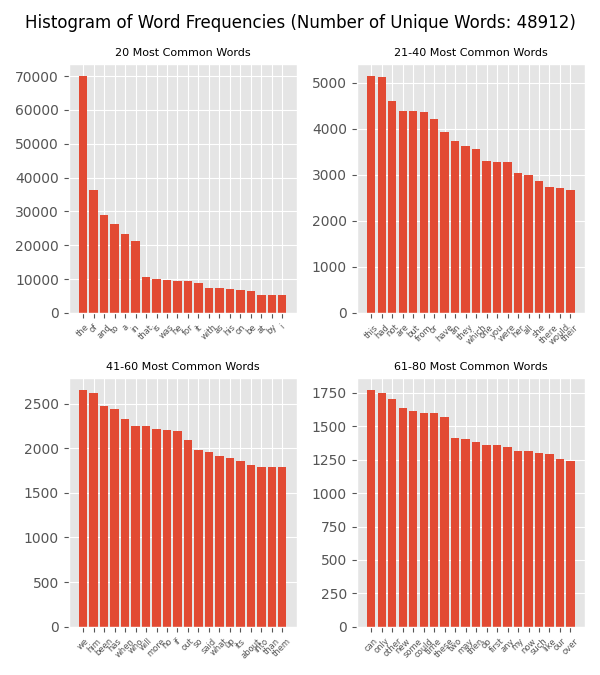
\includegraphics{word_frequency_distribution.png}    
    \caption{Number of instances of the 80 most common words in the data}
\end{figure}
\begin{figure}
    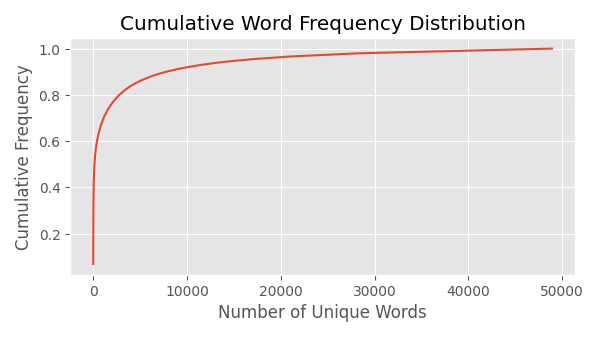
\includegraphics{cumulative_word_frequency.png}    
    \caption{Cumulative distribution function of word frequency}
\end{figure}
Furthermore, the word frequency cumulative distribution frequency suggests that at least 80\% of the instances is made out of the 10 thousands most common tokens. This supports our model architecture decision to limit our embedding to uniquely consider only those 10 thousands tokens, while regarding any other tokens (including those not in the dataset at all) as NULL\@.
\begin{figure}
    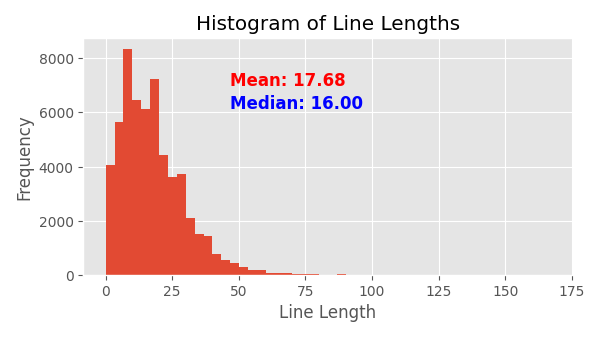
\includegraphics{length_distribution.png}    
    \caption{Length distribution of sentences in the dataset}
\end{figure}
Lastly, we explore the length of the lines. We see that the distribution is heavily concentrated around the low numbers, while having a long tail. This supports our model architecture decisions to train over eight token long sequences.
\subsection{Training Evaluation}
As expected, we see both the training loss and the test loss decrease as the training session progresses. After 100 epochs the test loss reaches a plateau so it seems like that any further improvement in training loss is appropriated to over-fitting (the model `memorizing' the dataset).
\begin{figure}
    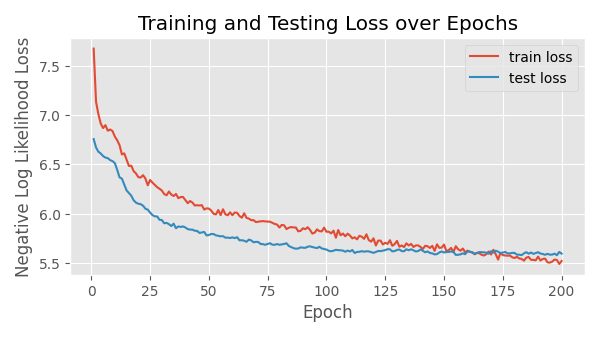
\includegraphics{loss-chart.png}
    \caption{Training and testing loss as the training session progresses}
\end{figure}
\section{Conclusions}
In this work, we implemented a simple RNN-based model to predict the next word
In this work, we sought out to predict the next word of a sentence, emulating a typical scenario of assisted typing over a touch device. We reframed this task as a statistical question of estimating the probabilistic \emph{language model} of the hypothetical user, and used machine-learning tools tackle this problem, as machine-learning turns large quantity of compute into a non-parametric estimate of statistical models. We wrote and shared the Python code over Pytorch that
trains and infers the trained model over arbitrary textual data. Finally, we executed this code over an example dataset and get examples:

\printbibliography
\end{document}
